\begin{recipe}
[ %
        preparationtime = {\SI{15}{\minute}},
        bakingtime={\SI{10}{\minute}},
        bakingtemperature={\protect\bakingtemperature{topbottomheat=\SI{175}{\celsius}}},
        portion = {\portion[Cookies]{some}},
        source = {LambMower}
    ]{Cookies}
    
    \begin{figure}[p]
    	\centering
    	\makebox[\textwidth][c]{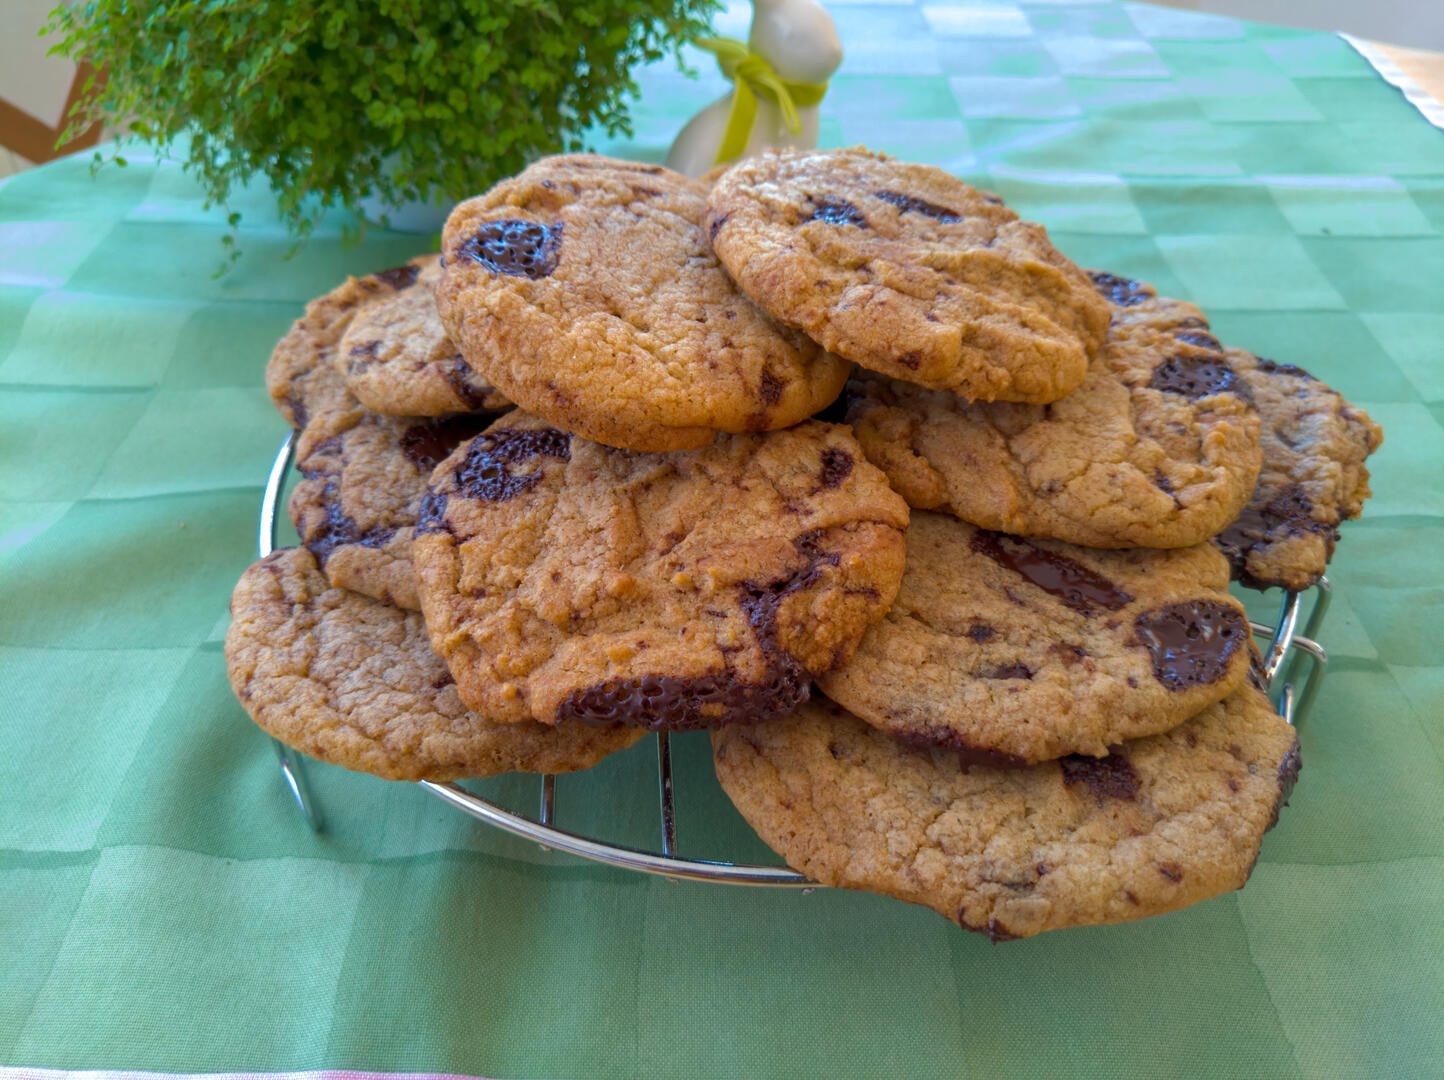
\includegraphics[height=\textheight]{cookies/IMG_20200424_132122.jpg}}
    \end{figure}
    
    \ingredients[10]{
        \SI{300}{\gram} & Butter \\
        \SI{2.25}{\deci\liter} & Sugar \\
        \SI{2.5}{\deci\liter} & Brown baking sugar \\
        2 & Eggs \\
        3\,tsp & Vanilla sugar \\
        \SI{7.5}{\deci\liter} & All-purpose Flour \\
        1\,tsp & Salt \\
        1\,tsp & Baking soda \\
        \SI{200}{\gram} & Chocolate of choice that’s been chopped chunky (I used baking milk chocolate)
    }

    \preparation{
        \step Melt the butter. 
        
        \vspace{1em}
        
        \step Whisk together the brown baking sugar, egg and vanilla sugar. 
        
        \step Add the butter once it’s not too warm (don’t want scrambled eggs) and whisk together. 
        
        \step Add salt and baking soda.
        
        \vspace{1em}
        
        \step Add the flour one cup at a time. Once the dough is like a giant fudgeball, add your chocolate to the dough and work that over.
        
        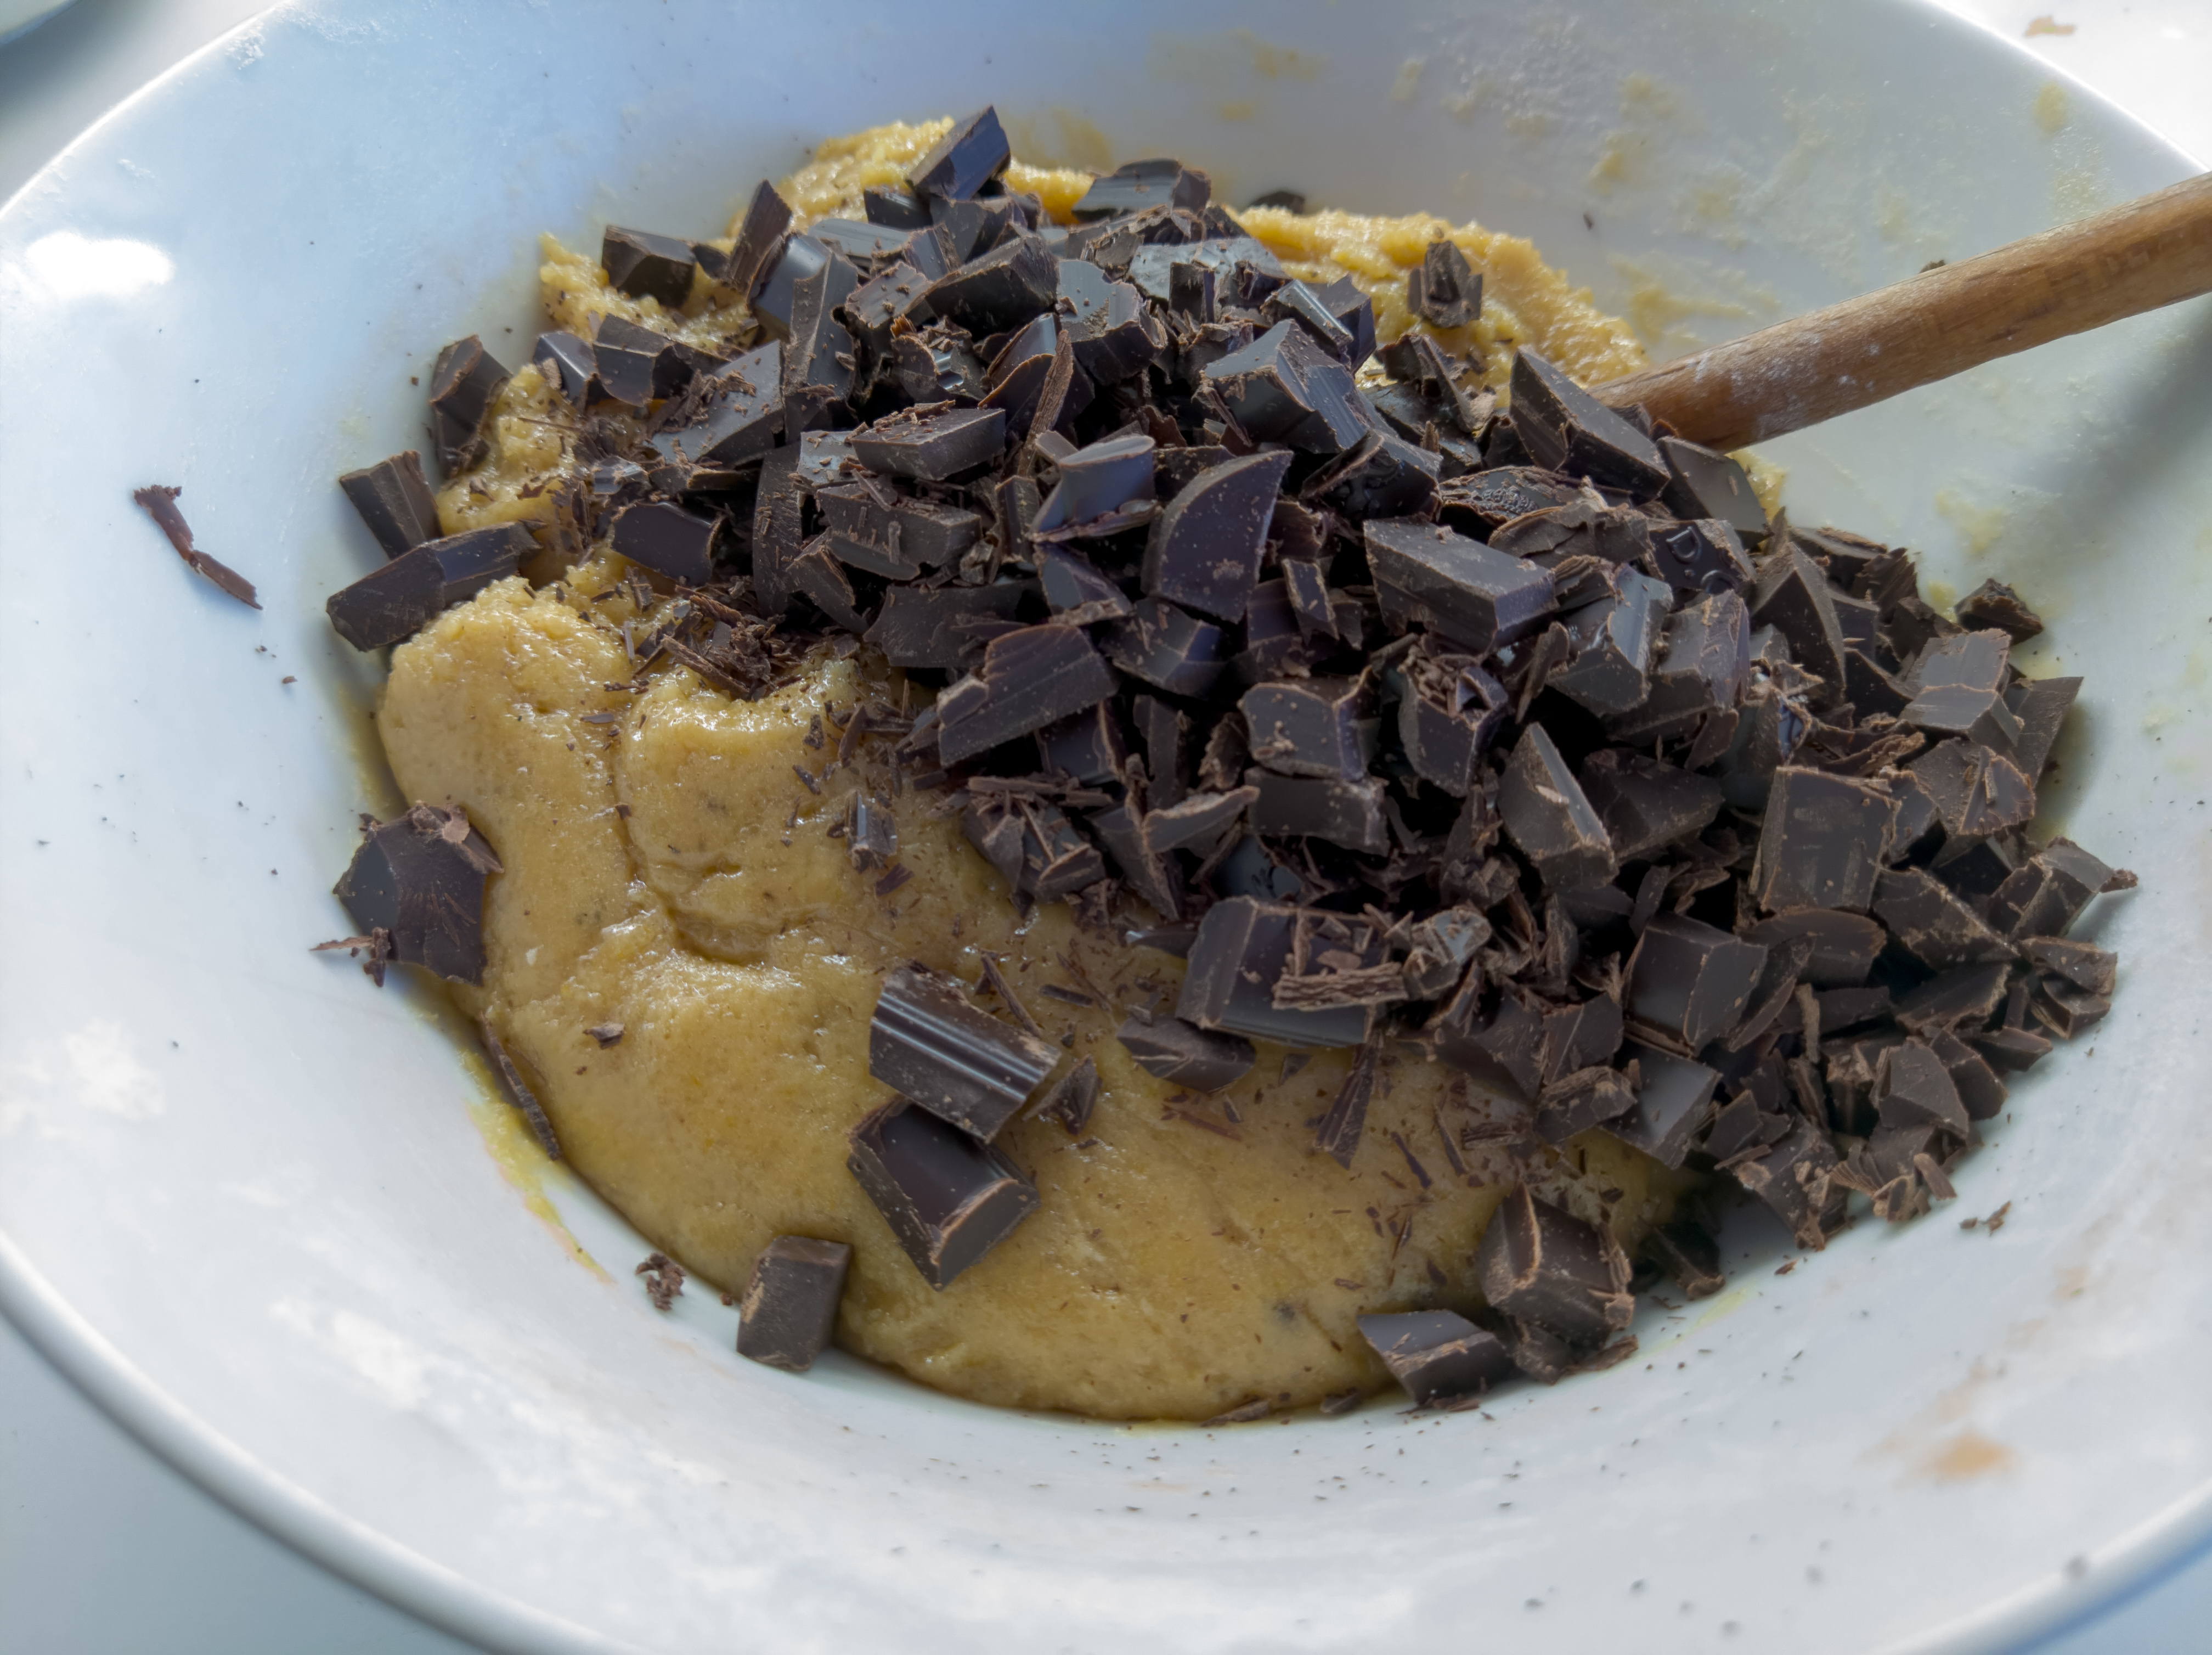
\includegraphics[width=0.525\textwidth]{cookies/IMG_20200424_115720.jpg}

        \step Form dough into balls -- about a tablespoon each -- and put them on a baking sheet covered in parchment paper. Press each ball down lightly.
        
        \step Put into oven at \SI{175}{\celsius} for \SI{10}{\minute}. Cookies are brittle when they come out, so wait a minute before transferring to a cooling rack.
    }
    
\end{recipe}